%!TEX program = lualatex
\documentclass[]{article}
\usepackage{longtable}

\input{preamble.tex}

\colorlet{accent}{jimp}

\title{Dokumentacja projektowa - Graficzny interfejs użytkownika dla wizualizacji grafów w języku Java}
\author{\authoricon Aleksander Jóźwik, Anastasiya Kryvetskaya}
\date{\dateicon \today}

\definecolor{zalety}{HTML}{a6d189}
\definecolor{wady}{HTML}{e78284}

\begin{document}
	\noindent
	\maketitle

	\tableofcontents
	\clearpage

    \section{Cel projektu}
	Celem projektu jest stworzenie graficznego interfejsu użytkownika w języku Java, który służy do przedstawienia rezultatu wizualizacji grafu i 
	daje możliwość podawania argumentów sterujących pracą algorytmów. Program bazuje na gotowej implementacji matematycznych algorytmów 
	do przetwarzania danych na konkretne pozycje elementów w przestrzeni.

	\section{Funkcjonalności programu}
	Program oferuje następujące funkcjonalności:
	\begin{enumerate}
		\item Wybór trybu wpisywania lub wczytywania i jeden z dostępnych formatów takich plików.
		\item Wybór algorytmu, który będzie obliczał współrzędne wierzchołków grafu.
		\item Możliwość zmiany palety kolorów grafu oraz rozmiaru promienia wierzchołków.
		\item Zapisywanie informacji o położeniu wierzchołków po ich rozmieszczeniu do pliku tekstowego lub binarnego.
		\item Graficzne przedstawienie elementów grafu: wierzchołki, krawędzie, wagi, etykiety.
		\item Możliwość poruszania się po przestrzeni na której znajduje się graf.
		\item Kontrola nad graficzną reprezentacją grafu: zmiana palety kolorów, ukrycie poszczególnych elementów.
		\item Pokazywanie aktualnego statusu działania programu: logi oraz błędy.
		\item Możliwość wyeksportowania graficznej reprezentacji grafu do pliku PNG.
	\end{enumerate}
	\clearpage
	
	\section{Graficzny interfejs i jego elementy}
	
    \begin{center}
	\begin{figure}[H]
    \centering
        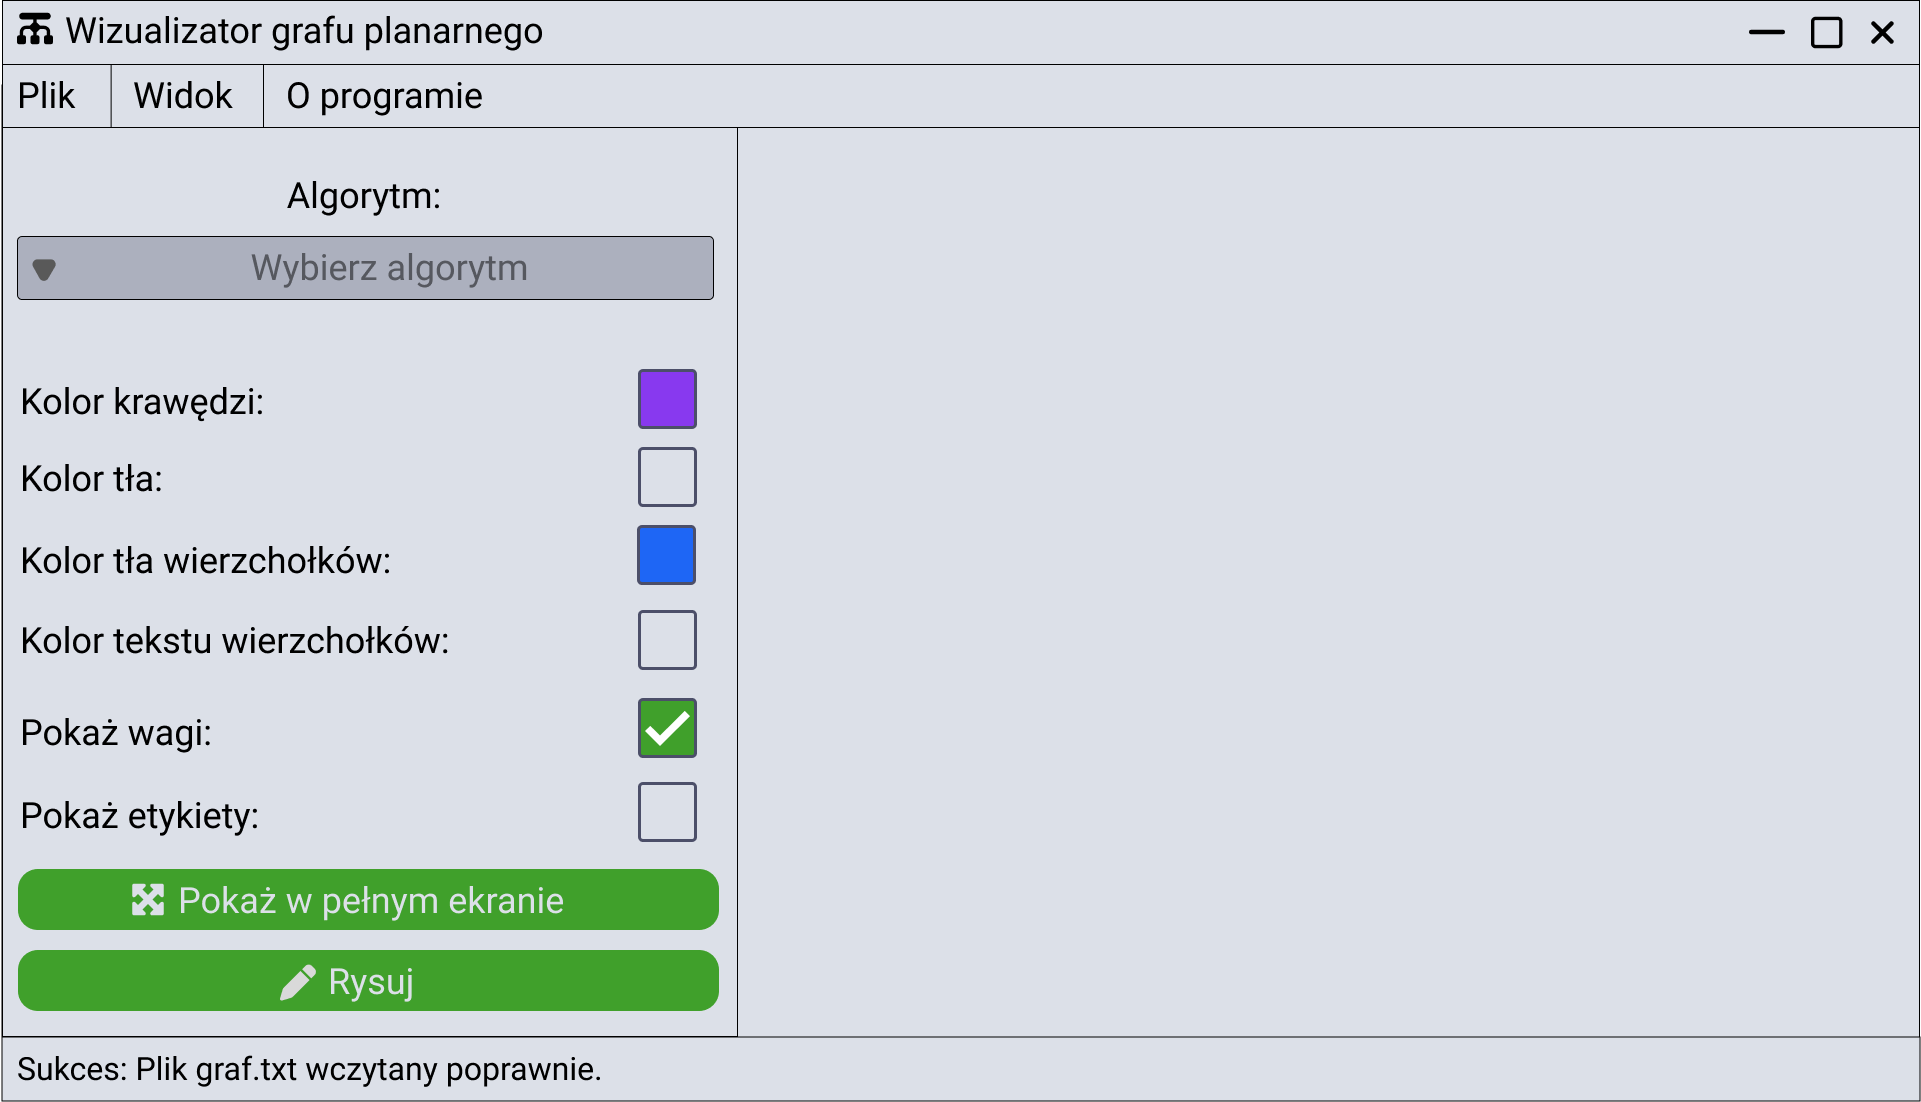
\includegraphics[width=1\textwidth]{assets/main.png}
    \caption{Graficzny interfejs}
    \label{fig:diagram_podzialu}
	\end{figure}
    \end{center}

	Interfejs składa się z 4 głównych elementów:
	\begin{itemize}
		\item Pasek menu
		\item Lewe okno służące do konfiguracji parametrów programu
		\item Prawe okno wyświetlające graf
		\item Pasek stanu na dole 
	\end{itemize}

	\clearpage
	\subsection{Pasek menu}
	Pasek menu składa się z 3 zakładek:
	\begin{itemize}
		\item Plik 
		\item Widok 
		\item O programie
	\end{itemize}

	\subsubsection{Zakładka Plik}

	\begin{figure}[H]
    \centering
		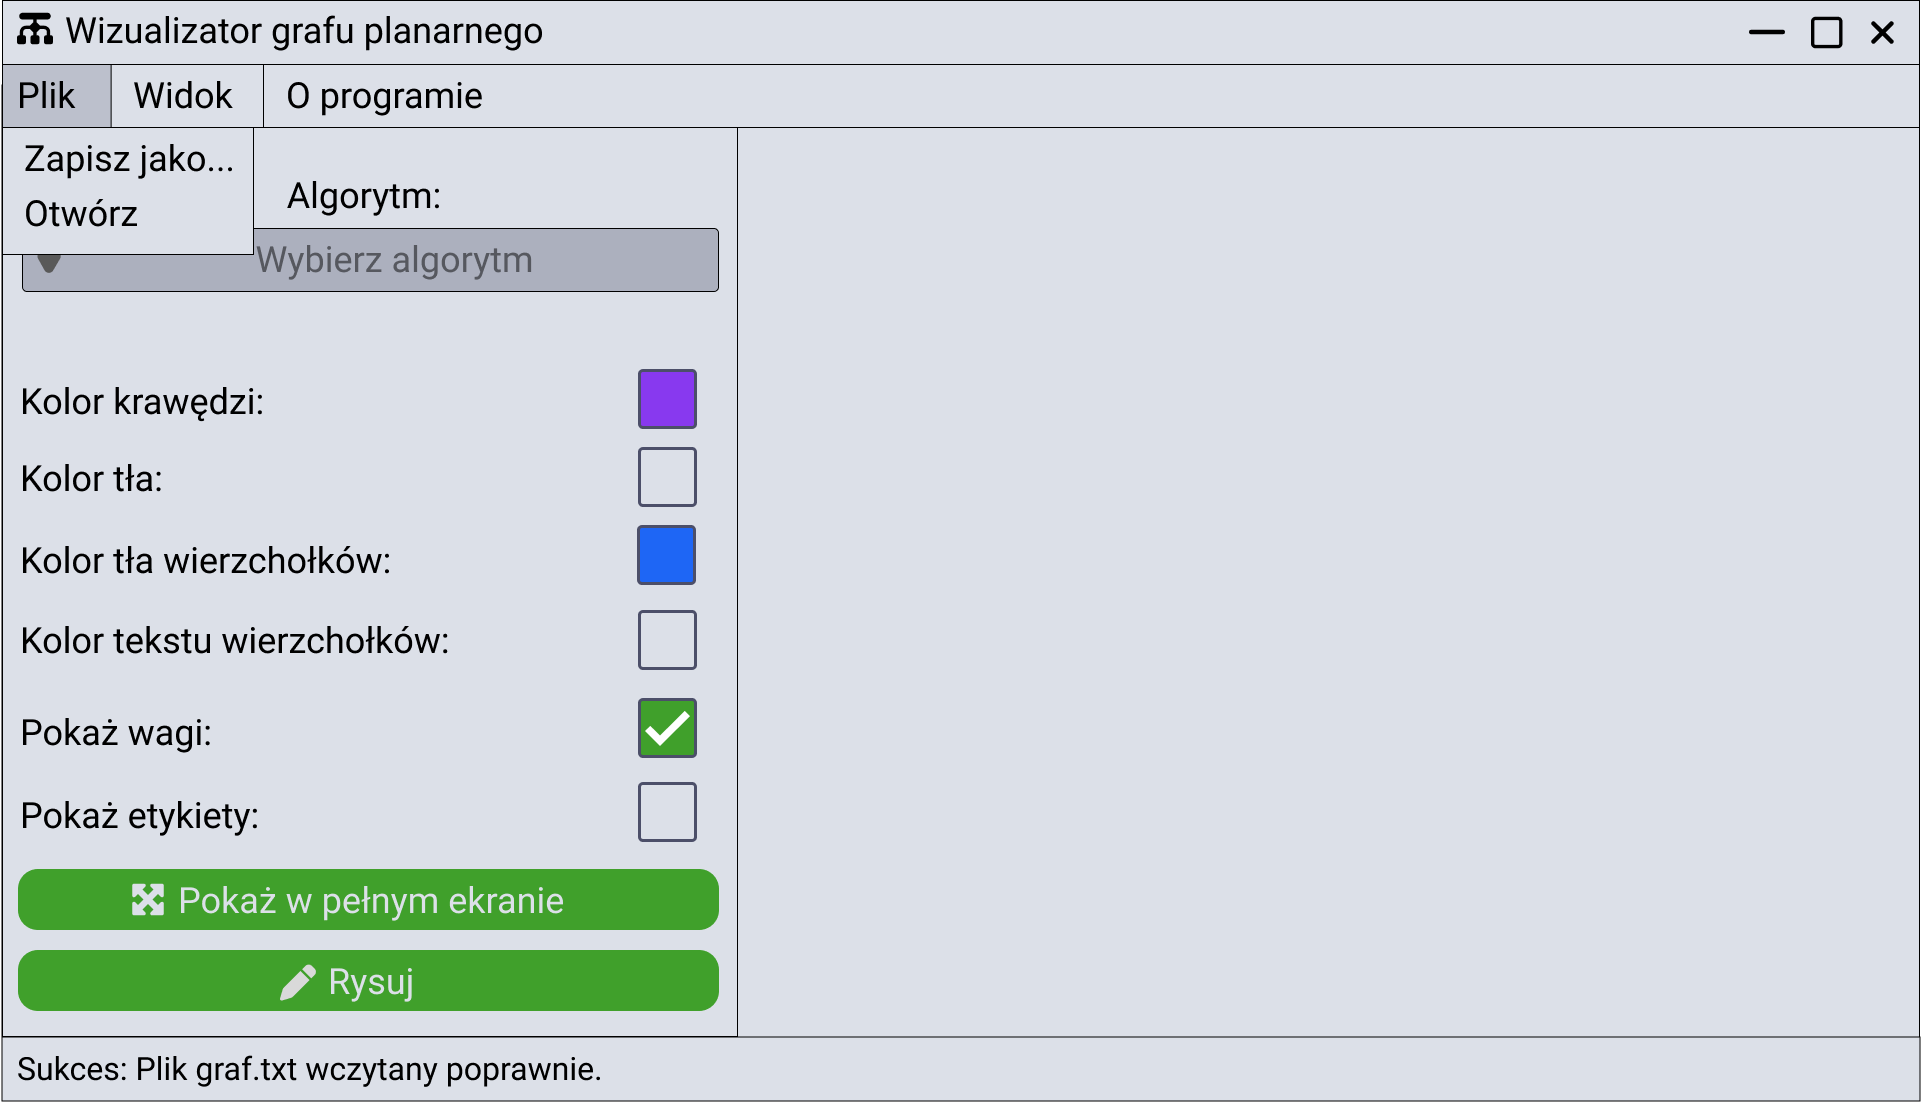
\includegraphics[width=0.8\textwidth]{assets/file_menu.png}
    \caption{Zakładka Plik}
    \label{fig:zakladka_plik}
	\end{figure}
	\textbf{Zakładka Plik} pozwala na zapis grafu do pliku PNG oraz na odczyt pliku tekstowego lub binarnego.
	\subsubsection{Zakładka Widok}
	\begin{figure}[H]
    \centering
		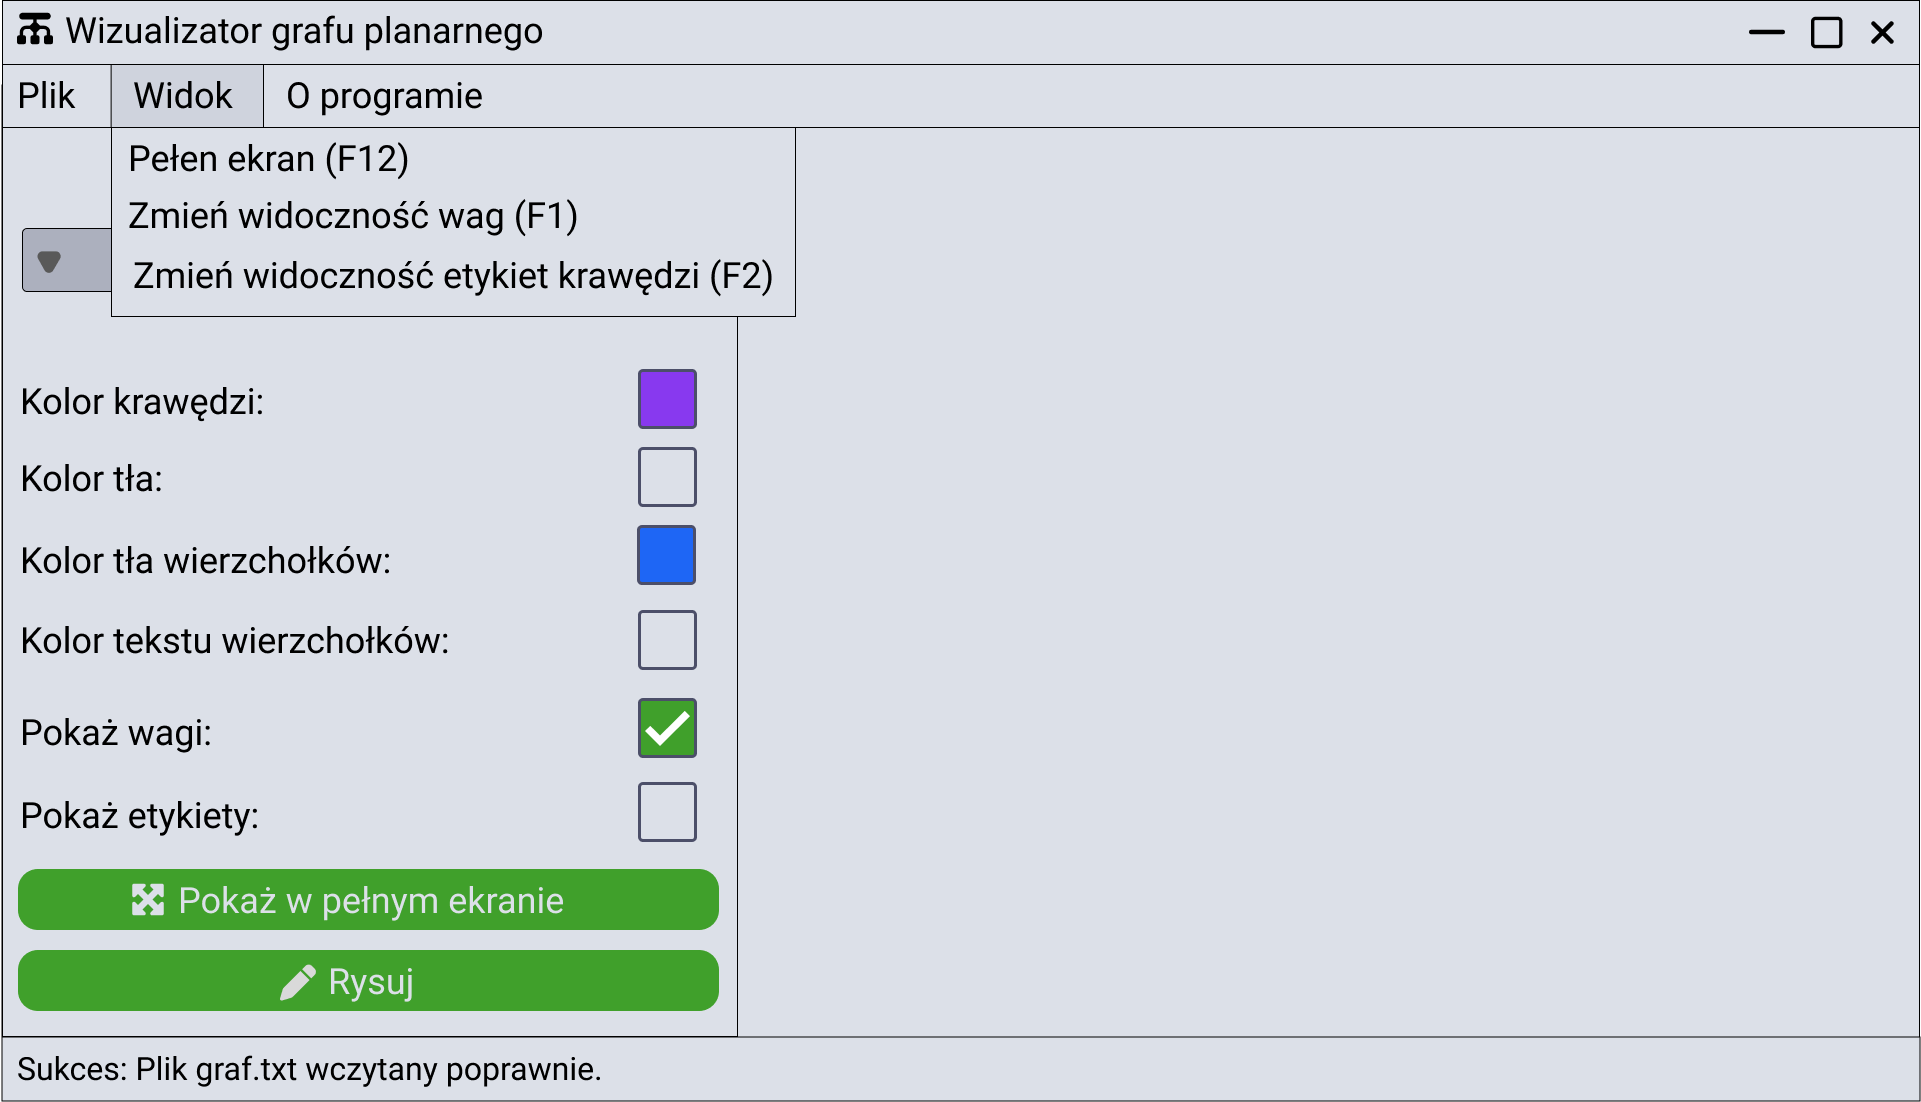
\includegraphics[width=0.8\textwidth]{assets/view_menu.png}
    \caption{Zakładka Widok}
    \label{fig:zakladka_widok}
	\end{figure}
	\textbf{Zakładka Widok} pozwala na obejrzenie grafu w pełnym ekranie, zmiany widoczności wag i etykiet krawędzi.

	\subsubsection{Zakładka O programie}

	\begin{figure}[H]
    \centering
		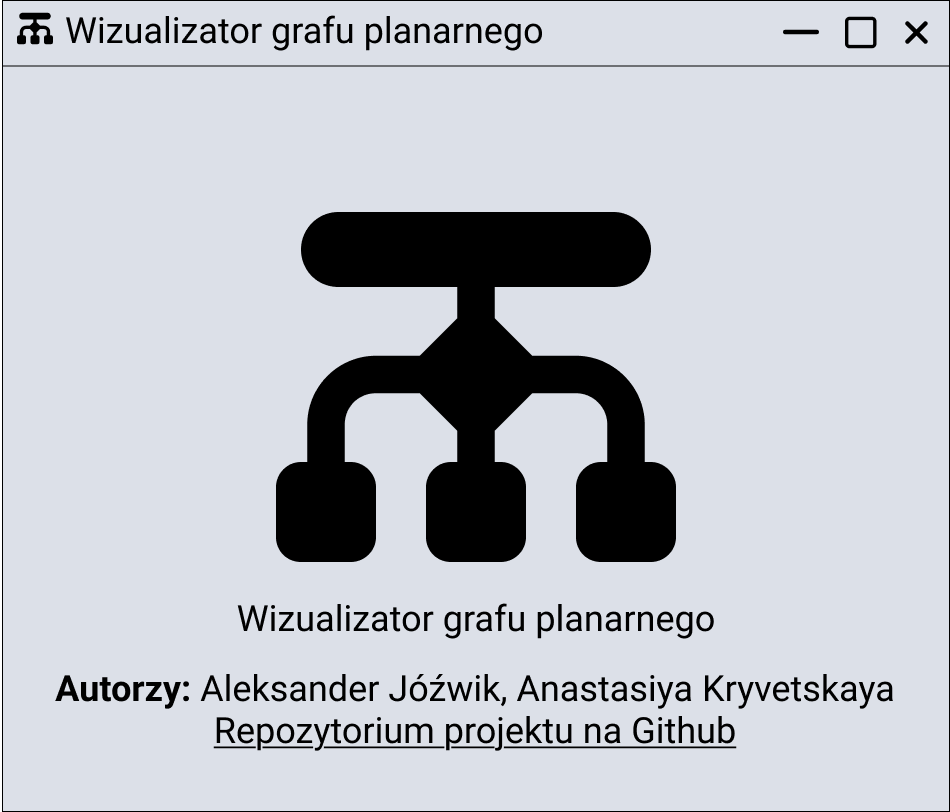
\includegraphics[width=0.5\textwidth]{assets/about.png}
    \caption{Okno O programie}
    \label{fig:okno_o_programie}
	\end{figure}

	Po naciśnięciu zakładki otwierane jest nowe okno, które informuje o autorach projektu i udostępnia link do repozytorium na Github.

	\subsection{Lewa część - Główne opcje wizualizacji}
	\begin{figure}[H]
    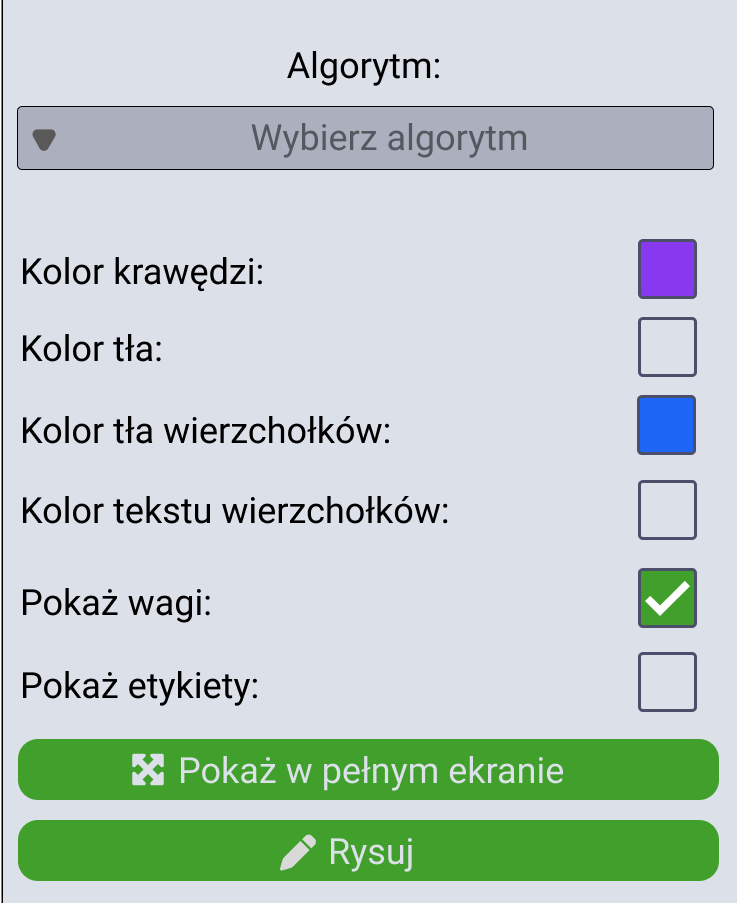
\includegraphics[width=0.8\textwidth]{./assets/menu_wizualizacji.png}
    \caption{Główne opcje wizualizacji}
    \label{fig:Górny pas menu}
	\end{figure}
	\textbf{Menu rozwijane} na górze pozwala wybrać jeden z dostępnych algorytmów do wykonania wizualizacji. Do momentu wybrania wyświetla się napis "Wybierz algorytm".
	\newline\textbf{Pola wyboru koloru} wywolują okna wyboru kolorów dla poszczególnych elementów grafu.

	Dolne \textbf{Pola wyboru} są odpowiedzialne za ukrywanie/pokazywanie wag oraz etykiet.


	\begin{figure}[H]
    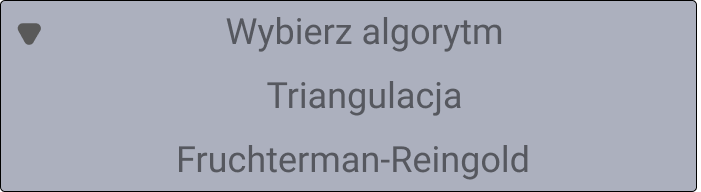
\includegraphics[width=0.8\textwidth]{./assets/Algorithm_Dropdown.png}
    \caption{Menu dla wyboru algorytmu}
    \label{fig:Menu dla wyboru algorytmu}
	\end{figure}
	\clearpage

Do wyboru dostępne 2 algorytmy: \textbf{Triangulacja} i \textbf{Fruchterman-Reingold}
\newline\textbf{Przycisk "Pokaż w pełnym ekranie"}  skaluje prawy obszar programu na całe okno.
\newline\textbf{Przycisk "Rysuj"} włącza algorytm.


	\subsection{Dolny pas menu - Status wykonania}
	W tym pasie znajduje się aktualny status wykonania wizualizacji. Opis możliwych błędów znajduje się w sekcji \ref{komunikaty_bledow}.
	W przypadku wystąpienia błędu pojawia się okno informujące o tym.
	\begin{figure}[H]
    
\includegraphics[width=0.8\textwidth]{./assets/blad.jpg}
    \caption{Status wykonania - błąd}
    \label{fig:okno - blad}
	\end{figure}

	\begin{figure}[H]
    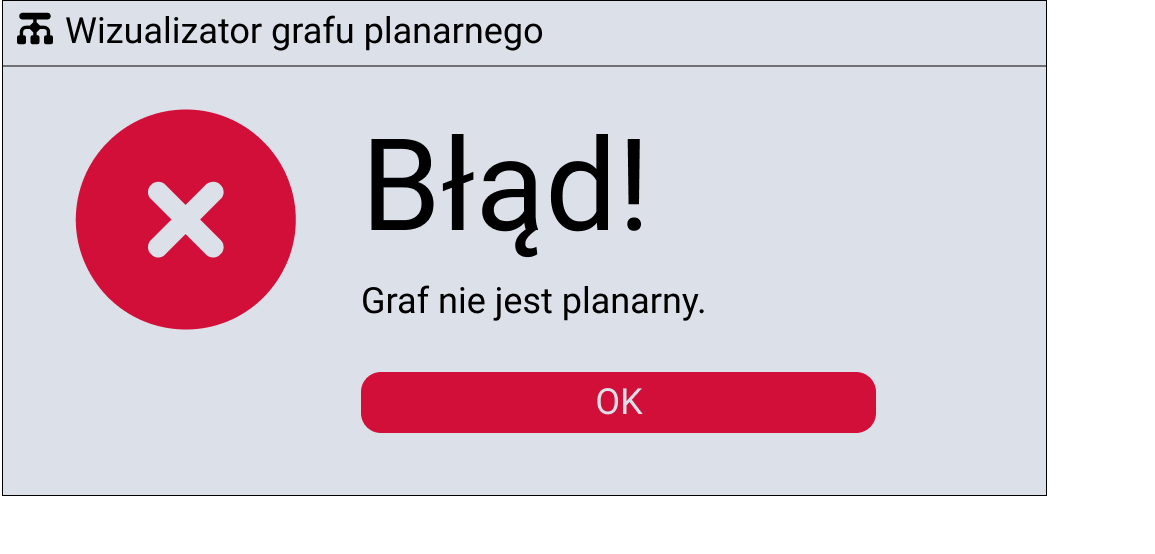
\includegraphics[width=0.8\textwidth]{./assets/okno_blad.png}
    \caption{Okno - błąd}
    \label{fig:okno - blad}
	\end{figure}
	
	\begin{figure}[H]
    
\includegraphics[width=0.8\textwidth]{./assets/sukces.jpg}
    \caption{Status wykonania - sukces}
    \label{fig:Status wykonania - bląd}
	\end{figure}
	
	\section{Format danych wejściowych}
	Dane wejściowe mają następujący format:
	\begin{mylisting}
<nazwa_krawędzi> <wierzchołek_A> <wierzchołek_B> <waga_krawędzi>	
	\end{mylisting}
	Na przykład:
	\begin{mylisting}
AB   1  2  1
BC   2  3  1
CD   3  4  1
DB   4  2  1.407
	\end{mylisting}

	\section{Komunikaty błędów}
	\label{komunikaty_bledow}

	\begin{tabularx}{\textwidth}{| X | X |}
		\hline
		Komunikat & Opis komunikatu\\
		\hline
		\texttt{BŁĄD: Nie udało się otworzyć pliku} & Wyświetlany, gdy nie udało się otworzyć wskazanego pliku.\\
		\hline
		\texttt{BŁĄD: Nie udało się zapisać pliku} & Wyświetlany, gdy nie udało się zapisać pliku.\\
		\hline
		\texttt{BŁĄD: Graf nie jest planarny} & Wyświetlany, gdy wczytany graf nie jest planarny. \\
		\hline
	\end{tabularx}

    \section{Architektura systemu}
    Struktura klas oraz przepływ sterowania w programie zostały zilustrowane za pomocą poniższych diagramów. 

    \framedfigure{assets/diagram_klas.png}{1\textwidth}{Diagram klas programu}{fig:class_diagram}

    \framedfigure{assets/schemat_blokowy.png}{0.5\textwidth}{Schemat blokowy działania programu}{fig:flowchart}
    
    \clearpage

    \subsection{Podział na moduły i wzorce projektowe}
    System został zaprojektowany w oparciu o podział na wyspecjalizowane pakiety klas, co zapewnia modularność i ułatwia ewentualną rozbudowę. Architektura programu luźno bazuje na koncepcji wzorca \textbf{MVC (Model-View-Controller)}:
    \begin{itemize}
        \item \textbf{Model} (logika i stan) -- reprezentowany głównie przez klasę \texttt{BackEnd}, która zarządza danymi (\texttt{Vertex}, \texttt{Edge}) oraz komunikacją z zewnętrznym procesem C.
        \item \textbf{Widok} (prezentacja) -- zbiór klas odpowiedzialnych za interfejs użytkownika (\texttt{GraphVisualizerUI}, \texttt{GraphCanvas}, paski menu), które prezentują dane graficzne bez ingerencji w ich strukturę.
        \item \textbf{Kontroler} (sterowanie) -- rozproszony w strukturach obsługi zdarzeń (np. \texttt{ActionListener}, \texttt{MouseListener}), które pośredniczą w przekazywaniu żądań z widoku do warstwy backendowej.
    \end{itemize}

    Ponadto interfejs graficzny w znacznym stopniu wykorzystuje wbudowany w technologię Java Swing wzorzec \textbf{Obserwator (Observer)}. Komponenty UI asynchronicznie nasłuchują na akcje użytkownika (np. kliknięcie przycisku rysowania czy odczytu pliku), po czym odpowiednio powiadamiają zarejestrowane obiekty obsługujące dane zdarzenie (Event Listeners).

    \section{Rdzeń programu}

    \subsection{Klasa  Main}
    Odpowiada za uruchomienie UI programu.
    \subsection{Klasa GraphVisualizerUI}
    Klasa ta stanowi główne okno aplikacji (\textit{Main Frame}). Dziedziczy po klasie \texttt{JFrame} i odpowiada za inicjalizację głównego interfejsu użytkownika, paska menu oraz rozmieszczenie głównych komponentów graficznych. Posiada dwie funkcje prywatne:
    \begin{itemize}
        \item initFrame -- ustawia właściwości okna tj. rozmiar, tytuł, układ rozmieszczenia elementów czy ikonę.
        \item initLayout -- dodaje pasek menu, lewe i prawe okno oraz pasek stanu.
    \end{itemize}
    Oraz funkcję publiczną \texttt{showErrorMessage}, która pozwala na wyświetlenie okna dialogowego z błędem oraz zmienia komunikat paska stanu.

    \subsubsection{Konstruktor \texttt{GraphVisualizerUI()}}
    Publiczny konstruktor klasy, który konfiguruje okno i buduje strukturę wizualną aplikacji.
    \textbf{Realizowane operacje:}
    \begin{itemize}
    \item Konfiguracja parametrów okna (tytuł, rozmiar, ikona).
    \item Inicjalizacja paska menu poprzez wstrzyknięcie obiektu klasy \texttt{TopMenuBar}.
    \item Wywołanie metod rozmieszczających panele boczne oraz obszar rysowania grafu.
    \end{itemize}

    \subsubsection{Struktura Interfejsu (Layout)}
    Główny interfejs został zorganizowany przy użyciu menedżera układu \texttt{BorderLayout} oraz komponentu \texttt{JSplitPane}.
    \begin{itemize}
    \item \textbf{SidebarPanel} (Zachód/Lewo): Panel boczny zawierający opcje sterowania wizualizacją.
    \item \textbf{GraphCanvas} (Centrum): Główny obszar roboczy służący do renderowania grafu.
    \item \textbf{StatusBar} (Południe/Dół): Pasek informacyjny wyświetlający aktualny stan programu.
    \end{itemize}

    \subsection{Klasa BackEnd}
    Odpowiada za warstwę logiczną aplikacji i komunikację z zewnętrznym programem obliczeniowym napisanym w języku C. Zarządza przechowywaniem wczytanego grafu (wierzchołków i krawędzi) oraz plikami wejściowymi i wyjściowymi.
    Posiada konstruktor \texttt{BackEnd()}, który inicjalizuje puste listy krawędzi i wierzchołków oraz ustawia domyślną ścieżkę pliku wyjściowego (\texttt{output.txt}).
    
    Klasa posiada następujące funkcje publiczne:
    \begin{itemize}
        \item setUI -- przypisuje referencję do głównego okna interfejsu (\texttt{GraphVisualizerUI}), co pozwala na m.in. wyświetlanie komunikatów o błędach.
        \item launchC -- odpowiada za przygotowanie odpowiednich argumentów i uruchomienie zewnętrznego programu w C (\texttt{a.out}) jako osobnego procesu, a następnie przechwytuje i wypisuje jego standardowe wyjście.
        \item setInputFile -- ustawia referencję do pliku wejściowego wybranego przez użytkownika.
        \item readInputFile -- parsuje zawartość pliku wejściowego, dodając odczytane obiekty do listy krawędzi (\texttt{edges}). Zwraca liczbę wczytanych elementów.
        \item readOutputFile -- parsuje zawartość pliku wyjściowego wygenerowanego przez algorytm, aktualizując współrzędne w liście wierzchołków (\texttt{vertices}). Zwraca liczbę poprawnie wczytanych wierzchołków.
        \item checkIfInputFileExists -- zwraca wartość logiczną informującą, czy plik wejściowy został wcześniej wybrany i załadowany.
    \end{itemize}

    \section{Klasy elementów UI}

    \subsection{Klasa GraphCanvas}

    Odpowiada za graficzne renderowanie struktury grafu oraz obsługę interakcji myszy. Posiada trzy funkcje publiczne i konstruktor:

    \begin{itemize}
        \item GraphCanvas(GraphVisualizerUI ui) -- konstruktor klasy; wiąże panel rysowania z kontekstem aplikacji, ustawia tło, marginesy, początkową pozycję kamery oraz rejestruje nasłuchiwacze zdarzeń myszy.
        \item resetCamera -- automatycznie kalkuluje granice grafu, centruje widok oraz dopasowuje współczynnik skalowania do bieżących wymiarów panelu.
        \item paintComponent -- nadpisuje natywną metodę rysującą komponent, odpowiadając za renderowanie krawędzi, wag, etykiet oraz wierzchołków z użyciem antyaliasingu.
        \item exportToPNG -- przechwytuje bieżący stan renderowania płótna i zapisuje go w formacie grafiki rastrowej PNG pod wskazaną ścieżką.
    \end{itemize}

    \subsection{Klasa TopMenuBar}
    Odpowiada za górny pasek menu. Posiada następujące funkcje prywatne:
    \begin{itemize}
        \item createStyledMenu -- tworzy nowe menu zgodnie z paletą kolorów.
        \item createStyledMenuItem -- tworzy nowy element menu zgodnie z paletą kolorów.
        \item saveFileAction -- otwiera okno dialogowe do zapisu pliku, wywołuje funkcje eksportującą graf do pliku PNG z klasy \texttt{GraphCanvas}, a następnie pokazuje komunikat w pasku stanu.
        \item openFileAction -- otwiera okno dialogowe do odczytu pliku, wywołuje funkcje wczytującą plik z klasy \texttt{BackEnd}, a następnie pokazuje komunikat w pasku stanu.
    \end{itemize}
    Oraz funkcje publiczne:
    \begin{itemize}
        \item getOpenFileName -- zwraca ścieżkę do aktualnie otwartego pliku.
        \item toggleSideBar -- służy do zmiany widoczności bocznego panelu. Dostępna pod skrótem klawiszowym \texttt{F12}.
        \item toggleWeights -- służy do zmiany widoczności etykiet wag. Dostępna pod skrótem klawiszowym \texttt{F1}.
        \item toggleLabels -- służy do zmiany widoczności etykiet krawędzi. Dostępna pod skrótem klawiszowym \texttt{F2}.
    \end{itemize}
    \subsection{Klasa SidebarPanel}
    Odpowiada za boczny panel pozwalający na konfigurację parametrów programu i uruchomienie wizualizacji. Posiada następujące funkcje:
    \begin{itemize}
        \item buildUI -- tworzy elementy UI w bocznym panelu.
        \item createColorSwatch -- tworzy przycisk odpowiadający za zmianę koloru.
        \item addPlainText -- służy do tworzenia zwykłego tekstu.
        \item addSectionTitle -- służy do tworzenia tekstu nagłówkowego.
        \item createRowWithLabel -- tworzy panel, w którym umieszcza etykietę i element podany jako argument.
        \item resetSettings -- przywraca domyślne wartości ustawień wizualizacji i odświeża interfejs.
    \end{itemize}
    \subsection{Klasa StatusBar}
   Odpowiada za dolny pasek stanu programu. Posiada jedną funkcję publiczną i konstruktor:
    \begin{itemize}
        \item setStatus -- ustawia i aktualizuje treść komunikatu wyświetlanego użytkownikowi na pasku stanu.
    \end{itemize}

    \subsection{Klasa AboutWindow}

    Odpowiada za wyświetlanie okna informacyjnego o programie (autorzy, wersja, link do repozytorium). Posiada dwie funkcje publiczne i konstruktor:

    \begin{itemize}
        \item centerThisText -- konfiguruje przekazaną etykietę tekstową, ustawiając jej kolor z motywu aplikacji oraz wyrównując ją do środka w osi X.
        \item createImageIcon -- wczytuje plik graficzny logo, skaluje go do wymiarów 120x120 pikseli z użyciem wygładzania i zwraca jako wycentrowany komponent etykiety.
    \end{itemize}

    \section{Klasy przechowujące dane}

    \subsection{Klasa Vertex} 
    Odpowiada za przechowywanie pojedynczego wierzchołka, czyli jego pozycji i identyfikatora.

    \subsection{Klasa Edge}
    Odpowiada za przechowywanie pojedynczej krawędzi, czyli jej nazwy, wagi i wierzchołka początkowego i końcowego.

    \section{Klasy dla ustawień programu}

    \subsection{Klasa VisualizationSettings}

    Odpowiada za przechowywanie obecnych ustawień programu (flagi określające widoczność etykiet krawędzi i wag oraz palete kolorów grafu). Klasa posiada jedynie konstruktor.

    \subsection{Klasa AppTheme}
    Odpowiada za zdefiniowanie domyślnej palety kolorów i czcionek.

    \section{Uwagi do zewnętrznego modułu obliczeniowego}
    Należy zaznaczyć, że dostarczony przez inny zespół moduł obliczeniowy w języku C nie w pełni realizował założenia opisane w jego dokumentacji. W szczególności program nie weryfikował, czy wprowadzony graf jest planarny oraz spójny. Ponadto implementacja algorytmu Fruchterman-Reingold nie funkcjonowała poprawnie, co wymagało z naszej strony ingerencji w kod źródłowy i naprawienia napotkanych błędów. Dodatkowym problemem, utrudniającym interpretację wyników, był brak odpowiedniej obsługi błędów. Komunikaty diagnostyczne zadeklarowane w dokumentacji modułu nie były generowane w przypadku niepowodzenia, co udowodniła weryfikacja z użyciem testowych zestawów danych dostarczonych przez autorów tamtego rozwiązania.
\end{document}
--comment

    Odpowiada za przechowywanie obecnych ustawień programu (flagi określające widoczność etykiet krawędzi i wag oraz palete kolorów grafu). Klasa posiada jedynie konstruktor.

    \subsection{Klasa AppTheme}
    Odpowiada za zdefiniowanie domyślnej palety kolorów i czcionek.

    \section{Uwagi do zewnętrznego modułu obliczeniowego}
    Należy zaznaczyć, że dostarczony przez inny zespół moduł obliczeniowy w języku C nie w pełni realizował założenia opisane w jego dokumentacji. W szczególności program nie weryfikował, czy wprowadzony graf jest planarny oraz spójny. Ponadto implementacja algorytmu Fruchterman-Reingold nie funkcjonowała poprawnie, co wymagało z naszej strony ingerencji w kod źródłowy i naprawienia napotkanych błędów. Dodatkowym problemem, utrudniającym interpretację wyników, był brak odpowiedniej obsługi błędów. Komunikaty diagnostyczne zadeklarowane w dokumentacji modułu nie były generowane w przypadku niepowodzenia, co udowodniła weryfikacja z użyciem testowych zestawów danych dostarczonych przez autorów tamtego rozwiązania.
\end{document}
--comment
